\section{Mesh Class Reference}
\label{classMesh}\index{Mesh@{Mesh}}
{\tt \#include $<$mesh.h$>$}

Collaboration diagram for Mesh:\nopagebreak
\begin{figure}[H]
\begin{center}
\leavevmode
\includegraphics[width=400pt]{classMesh__coll__graph}
\end{center}
\end{figure}
\subsection*{Public Member Functions}
\begin{CompactItemize}
\item 
{\bf Mesh} ()
\item 
{\bf $\sim$Mesh} ()
\item 
void {\bf init} ({\bf uint} {\bf ports}, {\bf uint} {\bf vcs}, {\bf uint} {\bf credits}, {\bf uint} {\bf buffer\_\-size}, {\bf uint} {\bf no\_\-nodes}, {\bf uint} {\bf grid\_\-size}, {\bf uint} {\bf links})
\item 
void {\bf setup} (void)
\item 
void {\bf connect\_\-interface\_\-processor} (void)
\item 
void {\bf connect\_\-interface\_\-routers} (void)
\item 
void {\bf connect\_\-routers} (void)
\item 
string {\bf print\_\-stats} (void)
\item 
void {\bf set\_\-max\_\-phy\_\-link\_\-bits} ({\bf uint} a)
\end{CompactItemize}
\subsection*{Public Attributes}
\begin{CompactItemize}
\item 
vector$<$ {\bf Router} $\ast$ $>$ {\bf routers}
\item 
vector$<$ {\bf Interface} $\ast$ $>$ {\bf interfaces}
\item 
vector$<$ {\bf Processor} $\ast$ $>$ {\bf processors}
\item 
vector$<$ {\bf GenericLink} $\ast$ $>$ {\bf link\_\-a}
\item 
vector$<$ {\bf GenericLink} $\ast$ $>$ {\bf link\_\-b}
\item 
unsigned long long int {\bf max\_\-sim\_\-time}
\end{CompactItemize}
\subsection*{Private Attributes}
\begin{CompactItemize}
\item 
{\bf uint} {\bf ports}
\item 
{\bf uint} {\bf vcs}
\item 
{\bf uint} {\bf credits}
\item 
{\bf uint} {\bf buffer\_\-size}
\item 
{\bf uint} {\bf no\_\-nodes}
\item 
{\bf uint} {\bf links}
\item 
{\bf uint} {\bf grid\_\-size}
\end{CompactItemize}


\subsection{Detailed Description}


Definition at line 94 of file mesh.h.

\subsection{Constructor \& Destructor Documentation}
\index{Mesh@{Mesh}!Mesh@{Mesh}}
\index{Mesh@{Mesh}!Mesh@{Mesh}}
\subsubsection[{Mesh}]{\setlength{\rightskip}{0pt plus 5cm}Mesh::Mesh ()}\label{classMesh_2af137f1571af89172b9c102302c416b}




Definition at line 23 of file mesh.cc.\index{Mesh@{Mesh}!$\sim$Mesh@{$\sim$Mesh}}
\index{$\sim$Mesh@{$\sim$Mesh}!Mesh@{Mesh}}
\subsubsection[{$\sim$Mesh}]{\setlength{\rightskip}{0pt plus 5cm}Mesh::$\sim$Mesh ()}\label{classMesh_5efe4da1a4c0971cfb037bd70304c303}




Definition at line 28 of file mesh.cc.

References interfaces, link\_\-a, link\_\-b, links, no\_\-nodes, processors, and routers.

\subsection{Member Function Documentation}
\index{Mesh@{Mesh}!connect\_\-interface\_\-processor@{connect\_\-interface\_\-processor}}
\index{connect\_\-interface\_\-processor@{connect\_\-interface\_\-processor}!Mesh@{Mesh}}
\subsubsection[{connect\_\-interface\_\-processor}]{\setlength{\rightskip}{0pt plus 5cm}void Mesh::connect\_\-interface\_\-processor (void)}\label{classMesh_9dfad9769d936905f5d8b0e4ffad6743}




Definition at line 80 of file mesh.cc.

References interfaces, link\_\-a, link\_\-b, no\_\-nodes, and processors.

Referenced by iris\_\-init(), and main().

Here is the caller graph for this function:\nopagebreak
\begin{figure}[H]
\begin{center}
\leavevmode
\includegraphics[width=187pt]{classMesh_9dfad9769d936905f5d8b0e4ffad6743_icgraph}
\end{center}
\end{figure}
\index{Mesh@{Mesh}!connect\_\-interface\_\-routers@{connect\_\-interface\_\-routers}}
\index{connect\_\-interface\_\-routers@{connect\_\-interface\_\-routers}!Mesh@{Mesh}}
\subsubsection[{connect\_\-interface\_\-routers}]{\setlength{\rightskip}{0pt plus 5cm}void Mesh::connect\_\-interface\_\-routers (void)}\label{classMesh_0bee0b7a3c9b621524748a97a3575db7}




Definition at line 96 of file mesh.cc.

References interfaces, link\_\-a, link\_\-b, no\_\-nodes, and routers.

Referenced by iris\_\-init(), and main().

Here is the caller graph for this function:\nopagebreak
\begin{figure}[H]
\begin{center}
\leavevmode
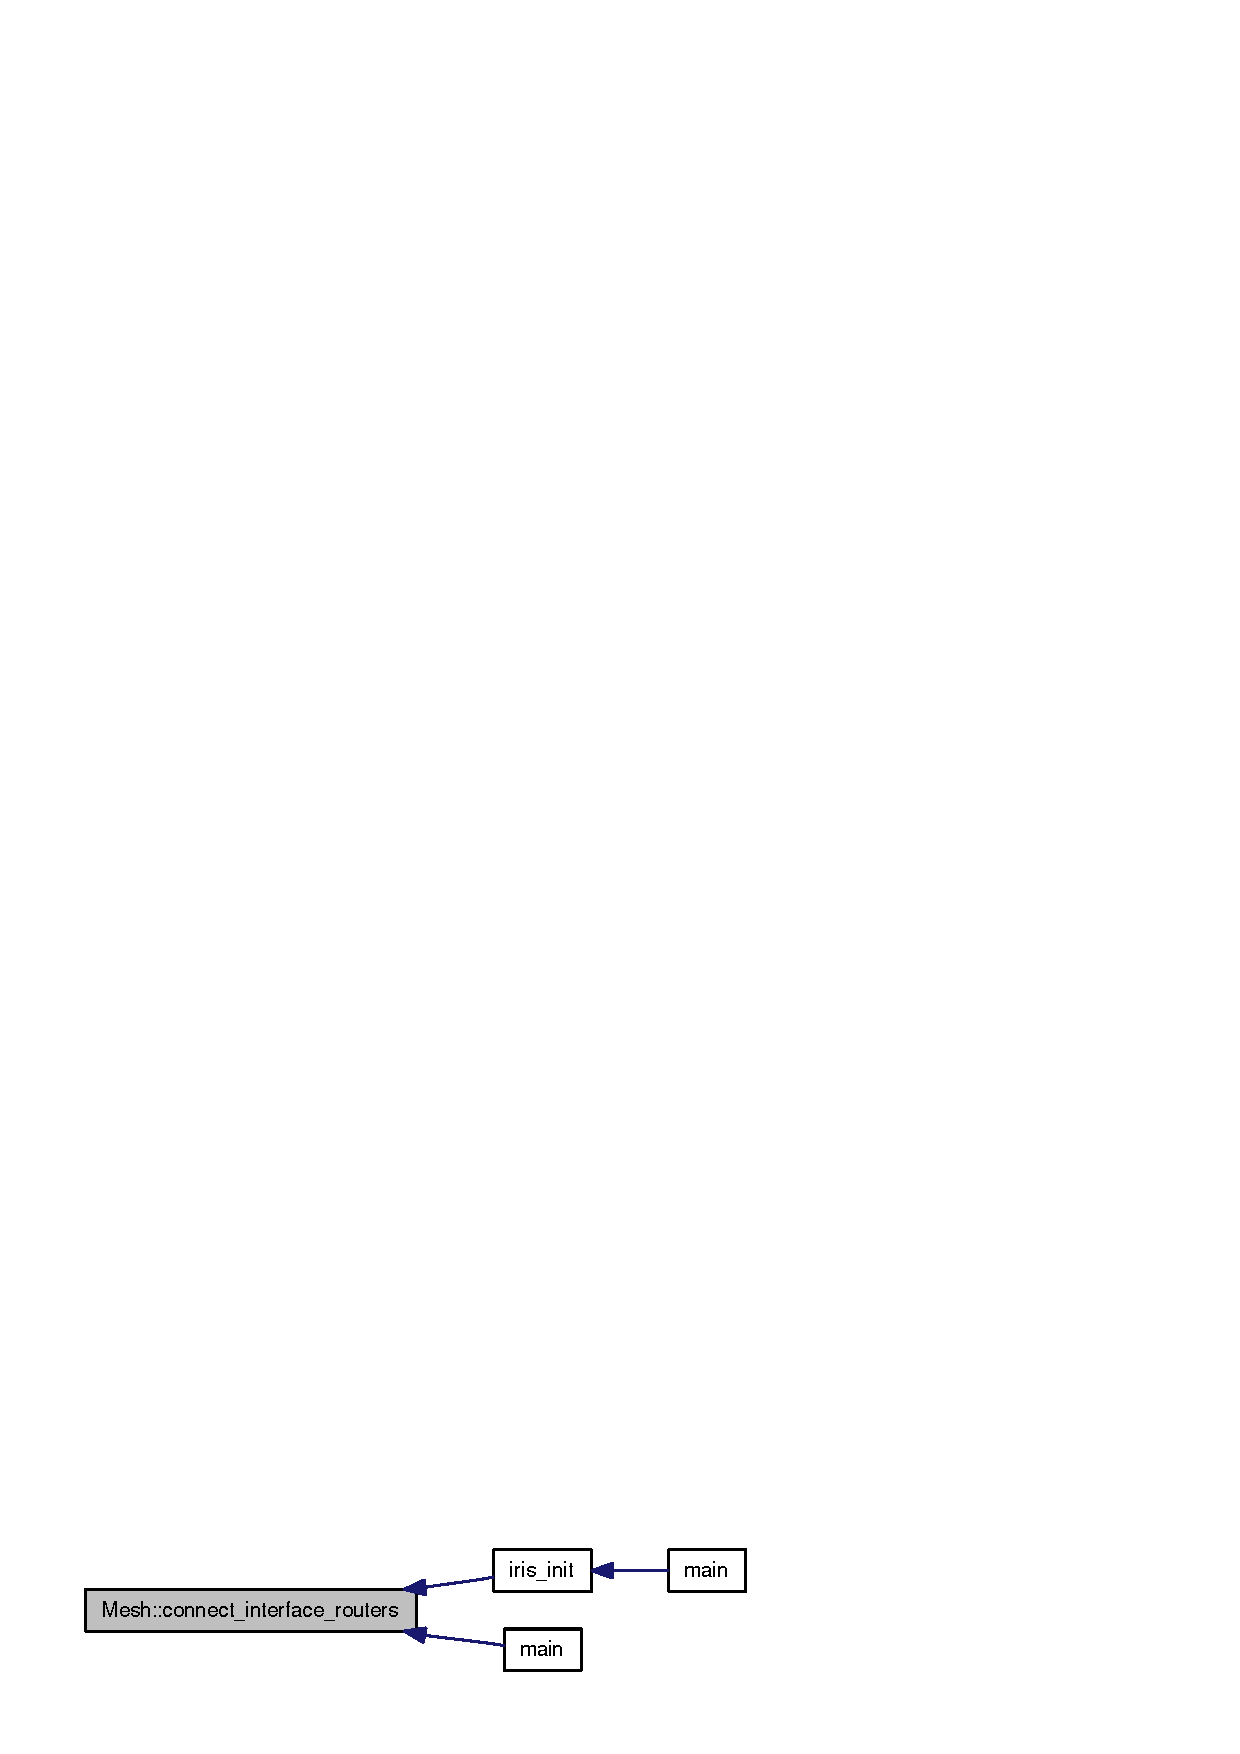
\includegraphics[width=181pt]{classMesh_0bee0b7a3c9b621524748a97a3575db7_icgraph}
\end{center}
\end{figure}
\index{Mesh@{Mesh}!connect\_\-routers@{connect\_\-routers}}
\index{connect\_\-routers@{connect\_\-routers}!Mesh@{Mesh}}
\subsubsection[{connect\_\-routers}]{\setlength{\rightskip}{0pt plus 5cm}void Mesh::connect\_\-routers (void)}\label{classMesh_fea2e233774ea469b02cff87afc336bc}




Definition at line 112 of file mesh.cc.

References grid\_\-size, link\_\-a, link\_\-b, links, no\_\-nodes, and routers.

Referenced by iris\_\-init(), and main().

Here is the caller graph for this function:\nopagebreak
\begin{figure}[H]
\begin{center}
\leavevmode
\includegraphics[width=159pt]{classMesh_fea2e233774ea469b02cff87afc336bc_icgraph}
\end{center}
\end{figure}
\index{Mesh@{Mesh}!init@{init}}
\index{init@{init}!Mesh@{Mesh}}
\subsubsection[{init}]{\setlength{\rightskip}{0pt plus 5cm}void Mesh::init ({\bf uint} {\em ports}, \/  {\bf uint} {\em vcs}, \/  {\bf uint} {\em credits}, \/  {\bf uint} {\em buffer\_\-size}, \/  {\bf uint} {\em no\_\-nodes}, \/  {\bf uint} {\em grid\_\-size}, \/  {\bf uint} {\em links})}\label{classMesh_678dc93df5115714b2d2e9a5932692db}




Definition at line 46 of file mesh.cc.

References buffer\_\-size, credits, grid\_\-size, links, no\_\-nodes, ports, and vcs.

Referenced by iris\_\-init(), and main().

Here is the caller graph for this function:\nopagebreak
\begin{figure}[H]
\begin{center}
\leavevmode
\includegraphics[width=131pt]{classMesh_678dc93df5115714b2d2e9a5932692db_icgraph}
\end{center}
\end{figure}
\index{Mesh@{Mesh}!print\_\-stats@{print\_\-stats}}
\index{print\_\-stats@{print\_\-stats}!Mesh@{Mesh}}
\subsubsection[{print\_\-stats}]{\setlength{\rightskip}{0pt plus 5cm}string Mesh::print\_\-stats (void)}\label{classMesh_eea84429f858784c6232e5633603fdf8}




Definition at line 58 of file mesh.cc.

References interfaces, no\_\-nodes, processors, and routers.

Referenced by main().

Here is the caller graph for this function:\nopagebreak
\begin{figure}[H]
\begin{center}
\leavevmode
\includegraphics[width=105pt]{classMesh_eea84429f858784c6232e5633603fdf8_icgraph}
\end{center}
\end{figure}
\index{Mesh@{Mesh}!set\_\-max\_\-phy\_\-link\_\-bits@{set\_\-max\_\-phy\_\-link\_\-bits}}
\index{set\_\-max\_\-phy\_\-link\_\-bits@{set\_\-max\_\-phy\_\-link\_\-bits}!Mesh@{Mesh}}
\subsubsection[{set\_\-max\_\-phy\_\-link\_\-bits}]{\setlength{\rightskip}{0pt plus 5cm}void Mesh::set\_\-max\_\-phy\_\-link\_\-bits ({\bf uint} {\em a})}\label{classMesh_592b6fea06d0348e4c18f2e43d8d051d}


\index{Mesh@{Mesh}!setup@{setup}}
\index{setup@{setup}!Mesh@{Mesh}}
\subsubsection[{setup}]{\setlength{\rightskip}{0pt plus 5cm}void Mesh::setup (void)}\label{classMesh_5c83ba3ef93b8ab63084b9c45082c7e9}




Definition at line 254 of file mesh.cc.

References buffer\_\-size, credits, interfaces, link\_\-a, link\_\-b, links, max\_\-sim\_\-time, no\_\-nodes, ports, processors, routers, and vcs.

Referenced by iris\_\-init(), and main().

Here is the caller graph for this function:\nopagebreak
\begin{figure}[H]
\begin{center}
\leavevmode
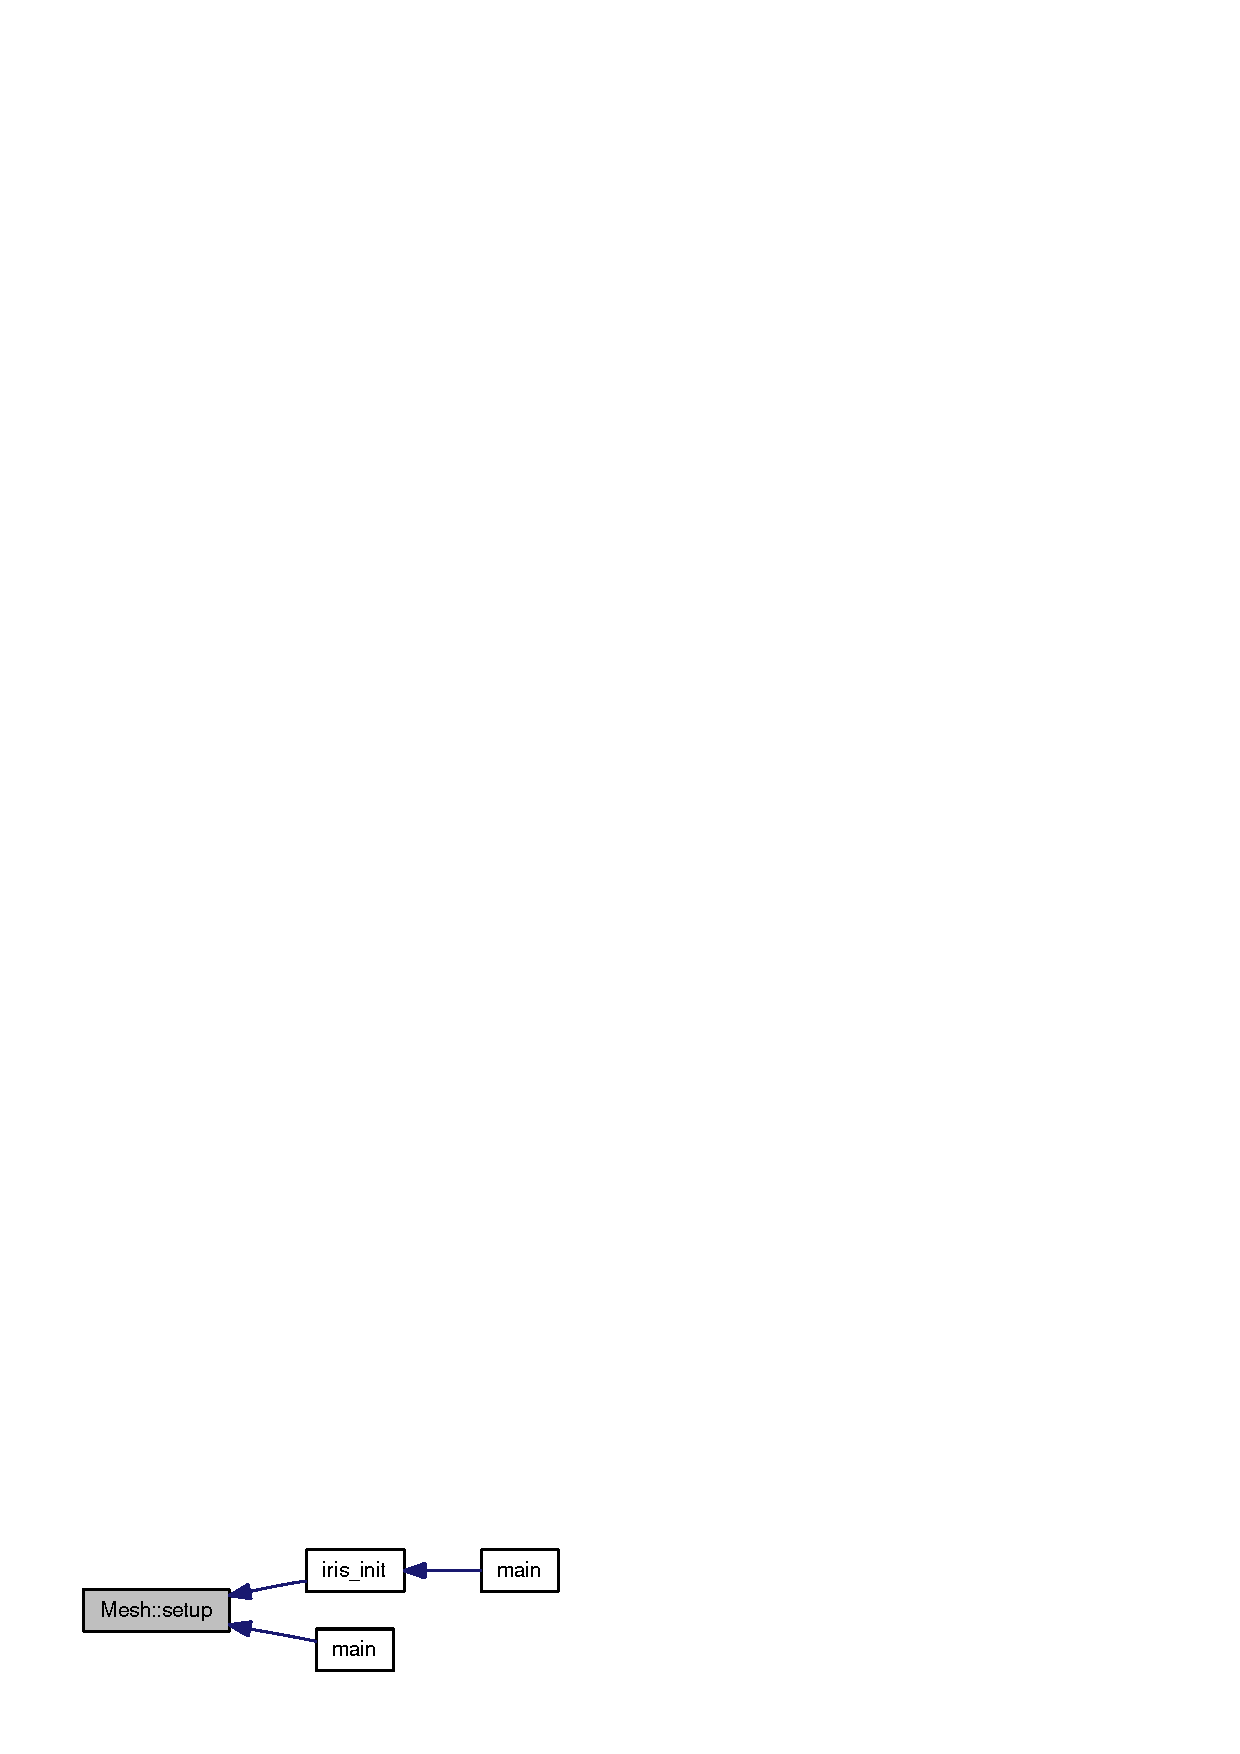
\includegraphics[width=136pt]{classMesh_5c83ba3ef93b8ab63084b9c45082c7e9_icgraph}
\end{center}
\end{figure}


\subsection{Member Data Documentation}
\index{Mesh@{Mesh}!buffer\_\-size@{buffer\_\-size}}
\index{buffer\_\-size@{buffer\_\-size}!Mesh@{Mesh}}
\subsubsection[{buffer\_\-size}]{\setlength{\rightskip}{0pt plus 5cm}{\bf uint} {\bf Mesh::buffer\_\-size}\hspace{0.3cm}{\tt  [private]}}\label{classMesh_f37fe94ec3960a966c8e740f8126aaf9}




Definition at line 120 of file mesh.h.

Referenced by init(), and setup().\index{Mesh@{Mesh}!credits@{credits}}
\index{credits@{credits}!Mesh@{Mesh}}
\subsubsection[{credits}]{\setlength{\rightskip}{0pt plus 5cm}{\bf uint} {\bf Mesh::credits}\hspace{0.3cm}{\tt  [private]}}\label{classMesh_2c9993f1d8e97db8abad7311664660c2}




Definition at line 119 of file mesh.h.

Referenced by init(), and setup().\index{Mesh@{Mesh}!grid\_\-size@{grid\_\-size}}
\index{grid\_\-size@{grid\_\-size}!Mesh@{Mesh}}
\subsubsection[{grid\_\-size}]{\setlength{\rightskip}{0pt plus 5cm}{\bf uint} {\bf Mesh::grid\_\-size}\hspace{0.3cm}{\tt  [private]}}\label{classMesh_843efbdd51b3f9ad9996a9e366e7df1d}




Definition at line 123 of file mesh.h.

Referenced by connect\_\-routers(), and init().\index{Mesh@{Mesh}!interfaces@{interfaces}}
\index{interfaces@{interfaces}!Mesh@{Mesh}}
\subsubsection[{interfaces}]{\setlength{\rightskip}{0pt plus 5cm}vector$<${\bf Interface}$\ast$$>$ {\bf Mesh::interfaces}}\label{classMesh_9ebde4264da1ba6e8f24bd2a24d05ef8}




Definition at line 100 of file mesh.h.

Referenced by connect\_\-interface\_\-processor(), connect\_\-interface\_\-routers(), iris\_\-init(), main(), print\_\-stats(), setup(), sim\_\-print\_\-stats(), and $\sim$Mesh().\index{Mesh@{Mesh}!link\_\-a@{link\_\-a}}
\index{link\_\-a@{link\_\-a}!Mesh@{Mesh}}
\subsubsection[{link\_\-a}]{\setlength{\rightskip}{0pt plus 5cm}vector$<${\bf GenericLink}$\ast$$>$ {\bf Mesh::link\_\-a}}\label{classMesh_25aed9e44396cd39a521e647d8e95ed2}




Definition at line 102 of file mesh.h.

Referenced by connect\_\-interface\_\-processor(), connect\_\-interface\_\-routers(), connect\_\-routers(), iris\_\-init(), main(), setup(), sim\_\-print\_\-stats(), and $\sim$Mesh().\index{Mesh@{Mesh}!link\_\-b@{link\_\-b}}
\index{link\_\-b@{link\_\-b}!Mesh@{Mesh}}
\subsubsection[{link\_\-b}]{\setlength{\rightskip}{0pt plus 5cm}vector$<${\bf GenericLink}$\ast$$>$ {\bf Mesh::link\_\-b}}\label{classMesh_8afcc482b97d3820e8249750c8a214c2}




Definition at line 103 of file mesh.h.

Referenced by connect\_\-interface\_\-processor(), connect\_\-interface\_\-routers(), connect\_\-routers(), iris\_\-init(), main(), setup(), sim\_\-print\_\-stats(), and $\sim$Mesh().\index{Mesh@{Mesh}!links@{links}}
\index{links@{links}!Mesh@{Mesh}}
\subsubsection[{links}]{\setlength{\rightskip}{0pt plus 5cm}{\bf uint} {\bf Mesh::links}\hspace{0.3cm}{\tt  [private]}}\label{classMesh_3ca6cc96b42524fcf15371eff8d29508}




Definition at line 122 of file mesh.h.

Referenced by connect\_\-routers(), init(), setup(), and $\sim$Mesh().\index{Mesh@{Mesh}!max\_\-sim\_\-time@{max\_\-sim\_\-time}}
\index{max\_\-sim\_\-time@{max\_\-sim\_\-time}!Mesh@{Mesh}}
\subsubsection[{max\_\-sim\_\-time}]{\setlength{\rightskip}{0pt plus 5cm}unsigned long long int {\bf Mesh::max\_\-sim\_\-time}}\label{classMesh_f81d45b09e24345365e6252a2243cc6b}




Definition at line 111 of file mesh.h.

Referenced by iris\_\-init(), main(), and setup().\index{Mesh@{Mesh}!no\_\-nodes@{no\_\-nodes}}
\index{no\_\-nodes@{no\_\-nodes}!Mesh@{Mesh}}
\subsubsection[{no\_\-nodes}]{\setlength{\rightskip}{0pt plus 5cm}{\bf uint} {\bf Mesh::no\_\-nodes}\hspace{0.3cm}{\tt  [private]}}\label{classMesh_df149d865bc81a734660461e97f9e9d8}




Definition at line 121 of file mesh.h.

Referenced by connect\_\-interface\_\-processor(), connect\_\-interface\_\-routers(), connect\_\-routers(), init(), print\_\-stats(), setup(), and $\sim$Mesh().\index{Mesh@{Mesh}!ports@{ports}}
\index{ports@{ports}!Mesh@{Mesh}}
\subsubsection[{ports}]{\setlength{\rightskip}{0pt plus 5cm}{\bf uint} {\bf Mesh::ports}\hspace{0.3cm}{\tt  [private]}}\label{classMesh_147329c914fbfb0f6ce733a4e3120bc6}




Definition at line 117 of file mesh.h.

Referenced by init(), and setup().\index{Mesh@{Mesh}!processors@{processors}}
\index{processors@{processors}!Mesh@{Mesh}}
\subsubsection[{processors}]{\setlength{\rightskip}{0pt plus 5cm}vector$<${\bf Processor}$\ast$$>$ {\bf Mesh::processors}}\label{classMesh_e3531860febe9e7194b5d44ac1c1b2d8}




Definition at line 101 of file mesh.h.

Referenced by connect\_\-interface\_\-processor(), iris\_\-init(), main(), print\_\-stats(), setup(), and $\sim$Mesh().\index{Mesh@{Mesh}!routers@{routers}}
\index{routers@{routers}!Mesh@{Mesh}}
\subsubsection[{routers}]{\setlength{\rightskip}{0pt plus 5cm}vector$<${\bf Router}$\ast$$>$ {\bf Mesh::routers}}\label{classMesh_da66e4e75f4e50237af30d495248cca2}




Definition at line 99 of file mesh.h.

Referenced by connect\_\-interface\_\-routers(), connect\_\-routers(), iris\_\-init(), main(), print\_\-state\_\-at\_\-deadlock(), print\_\-stats(), setup(), and $\sim$Mesh().\index{Mesh@{Mesh}!vcs@{vcs}}
\index{vcs@{vcs}!Mesh@{Mesh}}
\subsubsection[{vcs}]{\setlength{\rightskip}{0pt plus 5cm}{\bf uint} {\bf Mesh::vcs}\hspace{0.3cm}{\tt  [private]}}\label{classMesh_043374c0f6e25837894c5e24fd3aa57f}




Definition at line 118 of file mesh.h.

Referenced by init(), and setup().

The documentation for this class was generated from the following files:\begin{CompactItemize}
\item 
{\bf mesh.h}\item 
{\bf mesh.cc}\end{CompactItemize}
